\documentclass{uebungszettel}
\graphicspath{ . }

\newcommand{\N}{\mathbb{N}} % Natürliche Zahlen
\usepackage{tikz}
\usepackage{wrapfig}


\begin{document}
\pagestyle{empty}

\maketitle{Klasse 7./8. -- Gruppe 3}{7.\ und 21.\ Februar 2014}

Erinnerung: Die Menge der natürlichen Zahlen ist $\N = \{ 1, 2, 3, ... \}$.

\begin{aufgabe}{Geometrische Reihe}
  Zeige: Für alle natürlichen Zahlen $n \in \N$ gilt: \enspace $\sum\limits_{k=1}^n \frac{1}{2^k} = 1 - \frac{1}{2^n}$.
\end{aufgabe}

\begin{aufgabe}{Gauss-Formel}
  Zeige: Für alle natürlichen Zahlen $n \in \N$ gilt: \enspace $\sum\limits_{k=1}^n k = \frac{n \cdot (n+1)}{2}$.
\end{aufgabe}

\begin{aufgabe}{Induktionsungleichung}
  Zeige, dass für alle natürlichen Zahlen $n \geq 4$ gilt: \enspace $n! \geq 2^n \geq n^2$
\end{aufgabe}

\begin{aufgabe}{Pyramidalzahlen}
  Zeige: Für alle $n \in \N$ gilt: $\sum\limits_{k=1}^{n} k^2 = \frac{n \cdot (n+1) \cdot (2n+1)}{6}$
\end{aufgabe}

\begin{aufgabe}{Fibonacci-Zahlen}
  Die Fibonacci-Zahlen sind definiert durch
  \[ F_1 := 1, \quad F_2 := 1, \quad \quad F_{n+2} = F_{n+1} + F_n \text{ für $n \in \N$}. \]
  Zeige durch Induktion, dass für $n \in \N$ gilt:
  \[
    F_n = \frac{a^n - b^n}{\sqrt{5}}, \quad \text{wobei }
    a := \frac{1 + \sqrt{5}}{2}, \enspace
    b := \frac{1 - \sqrt{5}}{2}.
  \]
\end{aufgabe}

\begin{aufgabe}{Pascals Dreieck}
  In Pascals Dreieck ist jede Zahl die Summe der Zahlen darüber:

  \begin{center}
    \begin{tabular}{ccccccccc}
      & & & & 1 \\ \noalign{\smallskip\smallskip}
      & & & 1 & & 1 \\ \noalign{\smallskip\smallskip}
      & & 1 & & 2 & & 1 \\ \noalign{\smallskip\smallskip}
      & 1 & & 3 & & 3 & & 1 \\ \noalign{\smallskip\smallskip}
      1 & & 4 & & 6 & & 4 & & 1 \\ \noalign{\smallskip\smallskip}
    \end{tabular}
  \end{center}

  Zeige, dass für alle $n \in \N$ gilt: Die Summe der Zahlen in der $n$-ten Zeile ist $2^{n-1}$.
\end{aufgabe}

\newpage

\begin{aufgabe}{Trominos auf dem Schachfeld}
  Ein Tromino ist ein Stein, der zwei Schachbrettfelder breit und zwei Schachbrettfelder hoch ist und genau drei Schachbrettfelder überdeckt, also gewissermaßen ein $(2 \times 2)$-Quadrat, aus dem eine Ecke entfernt wurde. Zeige per Induktion, dass es für alle $n \in \N$ möglich ist, ein quadratisches Brett, das $2^n$ Felder breit und hoch ist, und aus dem eine Ecke entfernt wurde, mit Trominos zu belegen.
\end{aufgabe}

\begin{aufgabe}{Fehlerhafte Induktion}
  Wir behaupten, dass in einer Herde Pferde alle Tiere die gleiche Farbe haben. Unser "`Beweis"' für diese kühne Behauptung ist folgender:

  Wir führen Induktion über die Anzahl der Pferde in einer Herde durch.

  \emph{Induktionsanfang} ($n=1$): Klar: In einer Herde, die aus nur einem Pferd besteht, haben alle Tiere die gleiche Farbe.

  \emph{Induktionsschritt}: Angenommen, wir haben eine Herde mit $n+1$ Pferden. Wir greifen uns aus dieser Herde wahllos ein Tier $P_0$ heraus. Die verbleibenden Tiere bilden eine Herde bestehend aus $n$ Pferden. Nach Induktionsannahme haben sie alle die gleiche Farbe. Nun führen wir das Pferd $P_0$ wieder mit dem Rest der Herde zusammen und greifen uns ein anderes Pferd $P_1$ mit $P_0 \not= P_1$ heraus. Die verbleibenden Tiere bilden eine Herde mit $n$ Pferden, haben also wieder alle die gleiche Farbe. Damit wissen wir: Das Pferd $P_1$ hat die gleiche Farbe wie alle anderen Tiere außer $P_2$ und $P_2$ hat die gleiche Farbe wir alle anderen Tiere außer $P_1$. Somit hat auch $P_1$ die gleiche Farbe wie $P_2$ und somit hat die gesamte Herde die gleiche Farbe.

  Frage: Wo liegt der Fehler?
\end{aufgabe}

% \begin{aufgabe}{Fehlerhafte Induktion 2}
%   Achilles und eine Schildkröte liefern sich ein Wettrennen
% \end{aufgabe}

% 51. Methematik-Olympiade, 2. Stufe (Regionalrunde), Klasse 11-13, Aufgabe 511324
\begin{aufgabe}{Turnier}
  In einem Fechtturnier mit $2^n$ Teilnehmern kämpft jeder Fechter genau einmal gegen jeden anderen. Kein Kampf endet unentschieden. Eine Reporterin möchte nacheinander Einzelinterviews mit $n+1$ Fechtern führen. Diese sollen so ausgewählt werden, dass jeder interviewte Fechter gegen alle Fechter, die vor ihm interviewt wurden, gesiegt hat.

  Zeige zunächst, dass die Reporterin für $n=1$ und $n=2$ eine entsprechende Auswahl von Fechtern für die Interviews treffen kann. Zeige dann durch Induktion, dass dies auch für beliebige natürliche Zahlen $n$ möglich ist.
\end{aufgabe}

\begin{aufgabe}{Gesättigte gerichtete Graphen}
  \begin{wrapfigure}{r}{0.25\textwidth}
    \begin{center}
      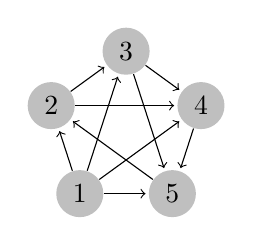
\begin{tikzpicture}[shorten >=1pt,->]
        \tikzstyle{vertex}=[circle,fill=black!25,minimum size=17pt,inner sep=0pt]

        \foreach \name/\angle/\text in {P-1/234/1, P-2/162/2, 
                                        P-3/90/3, P-4/18/4, P-5/-54/5}
          \node[vertex,xshift=6cm,yshift=.5cm] (\name) at (\angle:1cm) {$\text$};

        \foreach \from/\to in {1/2,2/3,3/4,4/5,1/5,1/3,2/4,3/5,1/4,5/2}
          { \draw (P-\from) -- (P-\to); }
      \end{tikzpicture}
    \end{center}
  \end{wrapfigure}

  Auf der rechten Seiten siehst du einen gesättigten gerichteten Graphen mit 5 Knoten (graue Kreise). Die Pfeile zwischen den Knoten werden auch {\em Kanten} genannt. Wir sagen, dass wir einen Knoten $B$ von einem anderen Knoten $A$ direkt erreichen können, wenn eine Kanten von A nach B verläuft (also die Pfeilspitze zu B zeigt). Ein Knoten $B$ kann von einem anderen Knoten $A$ in zwei Schritten erreicht werden, wenn es einen Knoten $C$ gibt, sodass $C$ von $A$ direkt erreichbar ist und $B$ von $C$ direkt erreichbar ist.

  Im Beispiel ist der Knoten $3$ vom Knoten $1$ in zwei Schritten erreichbar, aber andersrum der Knoten $1$ nicht vom Knoten $3$ in zwei Schritten erreichbar. Außerdem ist der Knoten $2$ von jedem anderen Knoten in höchstens zwei Schritten erreichbar.

  Zeige, dass es in jedem gesättigten gerichteten Graphen mit $n$ Knoten einen Knoten gibt, der von jedem anderen Knoten in höchstens zwei Schritten erreicht werden kann.
\end{aufgabe}

\end{document}
